% =====================================================================
% reference_draft.tex
%
% A REFERENCE MODEL, NOT THE MANUSCRIPT. Written by an AI assistant with
% access to the decision log, the frozen results and the figure/table
% package, so the authors can see one possible shape of the paper before
% writing their own. NONE OF THIS PROSE IS INTENDED FOR THE SUBMITTED
% PAPER. Read it, disagree with it, then write your own.
%
% Every number here is read from the frozen artifacts. Where a number is
% not in those artifacts it is marked \TODO.
%
% It is deliberately NOT cut to the 12-page PoPETs limit. Fitting it is a
% separate editorial pass; see paper/README.md for what to cut first.
% =====================================================================
\documentclass[sigconf,nonacm]{acmart}

\usepackage{booktabs}
\usepackage{graphicx}
\graphicspath{{../results/paper_package/figures/}{figures/}{./}}
\makeatletter
\providecommand\input@path{}
\g@addto@macro\input@path{{../results/paper_package/tables/}{tables/}}
\makeatother

% The 2027 PoPETs template provides these; stubs keep this draft compiling
% on its own. DELETE these stubs when moving into the real template.
\makeatletter
\@ifundefined{ethics}{\newenvironment{ethics}{\section*{Ethical Considerations}}{}}{}
\@ifundefined{openscience}{\newenvironment{openscience}{\section*{Open Science}}{}}{}
\@ifundefined{ai}{\newenvironment{ai}{\section*{AI Use}}{}}{}
\makeatother
\settopmatter{printacmref=false,printccs=false,printfolios=true}
\newcommand{\TODO}[1]{\textbf{[TODO: #1]}}
\newcommand{\FJ}{\ensuremath{F1_J}}
\newcommand{\FL}{\ensuremath{F1_L}}
\newcommand{\AJ}{\ensuremath{A_J}}
\newcommand{\AVJ}{\ensuremath{A_{VJ}}}
\newcommand{\VJ}{\ensuremath{V_J}}
\newcommand{\VL}{\ensuremath{V_L}}

\begin{document}

\title{What Survives Fragmentation: Measuring Source Linkage and Ordering
Leakage from Plaintext Fragments under a Modern Semantic Attacker}

% TODO authors: real names in the agreed order, affiliations, emails.
\author{Aiden J. Tejada}
\affiliation{\institution{TODO affiliation}\country{TODO country}}
\email{first.last@example.edu}
\author{TODO co-author}
\affiliation{\institution{TODO affiliation}\country{TODO country}}
\email{second.author@example.edu}

\begin{abstract}
Fragmentation protects sensitive associations by splitting data so that related
values are never visible together. Its unlinkability argument assumes the pieces
cannot be recombined. Prior work establishes that this assumption fails when
dependencies among the data permit recombination, and formalises the problem for
declared, attribute-level dependencies supplied to the protection design. We ask
whether the implicit dependencies carried by unconstrained natural-language
content constitute a comparable channel, in a setting where none of the physical,
visual, byte-level or window-overlap evidence that prior reconstruction work
relies on is available: the attacker sees plaintext fragments and nothing else.

We evaluate this with two games on frozen, pre-registered pools. Game~O gives the
attacker membership and asks only for order. Game~J withholds membership as well,
and asks for a partition into a known number of source documents with an ordering
inside each. The joint score factors exactly into a linkage component and a
conditional ordering component, so we can say which half fails.

On 46 pools of seven clinical case reports each, a one-shot generative attacker
reaches \FJ~$0.723$ against a trivial-strategy reference of $0.149$, recovering
most of the membership structure (\FL~$0.882$) and most of the relative order
($q=0.792$). Tested statistical and embedding attackers stay near the reference.
The effect is strongly conditional: on synthetic structured identifiers every
content-based attacker falls \emph{below} the reference and only a schema-aware
baseline exceeds it, and across a five-point granularity series on identical text
the null-adjusted score falls monotonically from $0.588$ at a sentence cut to
$0.016$ at one word. We also report what these scores mean literally: at the
sentence cut the attacker ends up holding $64.2\%$ of the document as one
contiguous stretch, but $37.7$ points of that are leaked by the cut alone before
the attacker does anything.

We claim no new reconstruction algorithm and no new problem: mixed-source
reconstruction, LLM-driven reconstruction and semantic linkage are all
established. The contribution is the measurement---a threat model and a metric
that separates linkage from ordering---and the finding that reconstructability
tracks the signal the fragments retain rather than their size alone.
\end{abstract}

\keywords{fragmentation, unlinkability, document reconstruction, large language
models, privacy measurement}

\maketitle

% =====================================================================
\section{Introduction}
\label{sec:intro}

Fragmentation is a standard answer to a specific privacy problem. Some
information is sensitive not because any single value is secret but because the
\emph{association} between values is: a date of birth is not identifying, a
postcode is not identifying, and a diagnosis may be public, but the three
together may identify a patient. Splitting the data so that constrained
attributes never appear together in the clear, encrypting what cannot be split,
is a well-developed design~\cite{ciriani2010}.

That design rests on an assumption, and the assumption has a known failure mode.
Requiring fragments to share no attributes is \emph{necessary but not
sufficient} for unlinkability, because dependencies among the data may allow the
fragments to be recombined~\cite{decapitani2014}. That result is formulated for
declared, attribute-level dependencies that are supplied to the protection design
as inputs. The question this paper asks is what happens when the dependency is
not declared and not declarable in that form---when it is simply the meaning of
the text.

\paragraph{The observation channel is the point.}
Reconstructing fragmented documents is not new, and we do not claim it. Classical
forensic work reassembles the fragments of a file using statistical models of
the bytes across a candidate boundary~\cite{shanmugasundaram2003}; later work
reassembles several files at once from a mixed pool~\cite{memonpal2006}; recent
work reconstructs several mechanically shredded documents simultaneously, at
scale, from the pixel content either side of a physical cut~\cite{paixao2020};
and multimodal models have been benchmarked on restoring a single shredded
document from image fragments~\cite{shredbench2026}. Reconstruction from very
small textual units is also established, for overlapping $n$-gram releases in
which consecutive windows share $n-1$ tokens~\cite{galle2015}.

Every one of those attackers has something our setting denies. Byte continuity,
pixel continuity across a physical cut, file headers that name the sources and
their starting fragments, window overlap that encodes adjacency directly---none
of it exists when the adversary holds a shuffled bag of plaintext pieces. What
remains is what the text says. Separately, large language models have been shown
to perform strong semantic linkage against pseudonymous
profiles~\cite{lermen2026}, which is a different task: matching identities, with
no ordering and no grouping of document fragments.

\paragraph{Contributions.}
We make two, and deliberately not more.

\begin{enumerate}
\item \textbf{A threat model and a measurement framework} for plaintext
fragmentation. Game~O isolates ordering leakage when membership is known; Game~J
measures joint source-association and ordering leakage when membership is
withheld. The id-level joint score factors exactly as $\FJ = \FL \cdot q$,
linkage times conditional ordering, so a failure can be attributed to a half
(\S\ref{sec:metrics}). No predecessor's metric separates these: the closest
reports a single immediate-adjacency rate over one global permutation, in which
the seam between two completed documents counts as correct because document
order is irrelevant there~\cite{paixao2020}.

\item \textbf{An empirical characterisation of when leakage occurs.}
Reconstructability tracks the signal the fragments retain. It is substantial for
clinical prose under the tested generative attacker, reduced by disruptive cuts,
qualitatively different for structured identifiers, and falls monotonically to
its random-shuffle reference across a five-point granularity series on identical
text.
\end{enumerate}

The attacker comparison is evidence for both of these, not a third contribution.
We report it as a comparison among \emph{tested} attackers, never as a claim
about the attainable performance of any attacker family.

% =====================================================================
\section{Background and Related Work}
\label{sec:related}

\subsection{Fragmentation for association privacy}
Confidentiality constraints model sensitive associations as sets of attributes
whose joint visibility must be prevented; a correct fragmentation is one in which
no fragment is a superset of a constraint and no two fragments share a cleartext
attribute, with attributes that are sensitive alone handled by
encryption~\cite{ciriani2010}. The second condition is an unlinkability
condition: it exists to stop an adversary joining two fragments on a shared
value. Subsequent work shows that condition is necessary but not sufficient once
data dependencies are present, and reformulates the design problem to account for
them~\cite{decapitani2014}. Our experiment is best read as an empirical probe of
a channel that family of models does not enumerate, not as an evaluation of any
particular scheme. We prove nothing and we refute nothing.

\subsection{Reconstruction from fragments}
\textbf{Classical reassembly.} Shanmugasundaram and Memon reassemble the
fragments of a single document by scoring candidate adjacency with a
context model built from the fragments themselves and searching for a
maximum-weight Hamiltonian path, rooted at a first fragment that is assumed known
from file headers~\cite{shanmugasundaram2003}. Their accuracy measure is the
proportion of adjacent pairs in the reassembly that are truly adjacent; it has no
membership term, so no number of theirs is comparable to ours. Notably, that
paper names the grouping of mixed-source fragments as a distinct prior stage and
leaves it outside its scope---though the problem did not stay open, as the next
paragraph records.

\textbf{Mixed-source reassembly.} Reassembling several sources at once from a
mixed pool is established. Memon and Pal reconstruct multiple fragmented image
files simultaneously, anchored at identified file
headers~\cite{memonpal2006}.\footnote{We were unable to obtain the primary text
of~\cite{memonpal2006} and describe it only at the level secondary sources
support. \TODO{obtain IEEE TIP 15(2):385--393 and confirm before camera-ready}}
Paixão et al.\ reconstruct several mixed strip-shredded text documents at once
with a self-supervised model of the pixel content around a shred boundary,
sweeping the number of mixed documents from one to one hundred and reporting
accuracy above $90\%$~\cite{paixao2020}. Their output is a single global
permutation---document membership is implicit in contiguous runs rather than
predicted---and their accuracy counts immediate adjacency, with the seam between
two completed documents counted as correct. We are therefore not first to
mixed-source reconstruction, and their headline number is not comparable to ours.

\textbf{Modern models.} ShredBench benchmarks multimodal models on restoring a
single shredded document from image fragments cut into 8, 12 or 16 irregular
pieces, scoring the recovered text with edit distance and finding performance
degrades as the piece count rises~\cite{shredbench2026}. Both LLM-driven
reconstruction and the study of fragmentation granularity are therefore
established; neither is claimed here. That work is also convergent evidence for
our granularity result in a different modality.

\textbf{Small units.} Gallé and Tealdi reconstruct text from the $n$-grams of a
corpus and their counts, modelling the problem as a de~Bruijn graph in which
Eulerian cycles are plausible reconstructions~\cite{galle2015}. Order-$n$
$n$-grams overlap by $n-1$ tokens, so adjacency is present in the released data;
our fragments are a disjoint partition and share nothing, which is a difference
in the observation model rather than in the size of the unit.

\subsection{Semantic linkage with language models}
LLM pipelines combining feature extraction, embedding retrieval and model
reasoning perform large-scale deanonymization of pseudonymous profiles,
substantially outperforming classical feature-based matching, in a closed-world
setting whose difficulty parameters the authors vary
explicitly~\cite{lermen2026}. We do not claim to have discovered semantic
linkage. That work matches identities; it does not order or group document
fragments. Its closed-world design is also the precedent for ours---and, as
\S\ref{sec:limitations} records, for a limitation we do not discharge.

% =====================================================================
\section{Threat Model, Games and Metrics}
\label{sec:model}

\subsection{Setting}
A fragmentation scheme cuts each document into contiguous pieces and withholds
their order and grouping. We give the adversary the \emph{plaintext} pieces
deliberately: the question is what order- and membership-deprivation alone
withholds, independent of any encryption or hardware layer. A scheme that resists
reassembly on plaintext resists it a fortiori when the pieces are also encrypted.

\subsection{Game J: joint membership and order}
The attacker receives all fragments of a pool of $N=7$ source documents, with
fragment text, masked aliases, knowledge of $N$, and a shuffled presentation. It
does not receive true memberships, true order, true group sizes, or the raw
fragment identifiers. It must return a partition into exactly $N$ ordered groups,
using every fragment once. It is denied auxiliary context: no web access, no
external corpus, no named-record set.

\subsection{Game O: ordering with membership given}
The same, for one document whose membership is given; the attacker is asked only
for the order. Game~O isolates what fragmentation removes from \emph{order};
Game~J adds the source-association problem on top.

\subsection{What the attacker is \emph{not} told, and what it is}
Game~J is attacker-favourable relative to any real deployment, in four ways that
we state rather than bury: every fragment of every pooled document is present;
every represented source is complete; the number of sources is known; and the
pool is small ($\approx$140--540 fragments) rather than a global population of
unknown size with partially represented sources. \textbf{This study does not
evaluate that deployment-level partial-compromise problem.} Our numbers
characterise what an attacker with complete, small-pool access achieves. They do
not estimate leakage under partial compromise or global shuffling, and we do not
extrapolate to it.

\subsection{Metrics}
\label{sec:metrics}
An answer is a partition with an order inside each group. We score the
\emph{ordered pairs} it implies: for every pair $(a,b)$ placed in the same group
with $a$ before $b$, the pair is correct when $a$ and $b$ truly share a document
and $a$ truly precedes $b$. \FJ\ is the $F_1$ of that set against the truth.
Discarding direction gives \FL, the linkage component. Writing $C$ for the pairs
that are both co-clustered and correctly directed and $K$ for those co-clustered
at all, the two scores share a denominator, so
\[
  \FJ \;=\; \FL \cdot q, \qquad q = C/K,
\]
exactly, by construction rather than as an approximation. $q$ is the conditional
ordering accuracy: the share of correctly grouped pairs that also point the right
way. It is aggregated as $\sum C / \sum K$ over pools, and is undefined rather
than zero when $K=0$.

\paragraph{Reference points, and what they are not.}
The reference we normalise against is the expected score of putting every
fragment in one group in a random order, computed in closed form from the pool's
group sizes. For a pool with document sizes $m_d$, writing
$T=\sum_d \binom{m_d}{2}$ and $P=\binom{M}{2}$ for $M$ fragments,
$\mathbb{E}[\FL] = 2T/(P+T)$ and $\mathbb{E}[\FJ] = T/(P+T)$. The advantage is
$\AJ = (\FJ - b_J)/(1 - b_J)$, computed per pool and then averaged---normalising
grand means is a different quantity.

This is a \textbf{trivial-strategy reference, not a floor}: an all-singleton
answer scores $0$, which is lower. It is also not the chance level of a
\emph{legal} answer, because one bucket is not a partition into $N$ groups. We
report a legal random attacker separately in \S\ref{sec:adjacency} and show the
one-bucket figure overstates the floor by roughly a factor of two.

\paragraph{Visible-text metrics.}
At fine granularity many fragments share their surface text, and swapping the
hidden identifiers of two identical tokens is invisible to any attacker yet
penalised by an identifier-level scorer. For the granularity experiments we
therefore score only what is observable: the visible whitespace-token sequences.
\VL\ is the maximum over one-to-one assignments of predicted groups to true
documents of the summed multiset token overlap, normalised by the true token
count; \VJ\ replaces multiset overlap with token-level longest common
subsequence. Because \VL\ and \VJ\ are maximised over \emph{separate}
assignments, their ratio is a diagnostic and is \emph{not} the visible analogue
of $q$. Advantage is taken against a permutation null---labels permuted into the
true per-document fragment counts, 10{,}000 draws per pool---giving
$\AVJ = (\VJ - \overline{\VJ^{\text{null}}})/(1-\overline{\VJ^{\text{null}}})$.

\paragraph{Statistics.}
Percentile bootstrap, 10{,}000 resamples, seed 42; pools are the unit for
Game~J and documents for Game~O; paired resampling carries both conditions.
Paired differences also report an exact two-sided sign test. We do not adjust for
multiplicity and say so wherever a family of comparisons is reported.

% =====================================================================
\section{Experimental Setup}
\label{sec:setup}

\subsection{Corpora}
\textbf{Clinical prose.} 500 PMC Open Access clinical case reports,
case-narrative paragraphs only, commercial-use Creative Commons licences only,
published after the attacker model's stated training cutoff and verified
post-cutoff for all 500 documents. Roughly 315k words in 16{,}524 sentence
fragments. Post-cutoff publication is evidence against ordinary training-set
contamination; it is not a proof that no exposure occurred.

\textbf{Structured identifiers.} 500 synthetic records from a seeded generator,
one fragment per field. These are not derived from any person.
\S\ref{sec:synthetic} argues what they do and do not support.

\subsection{Cuts and conditions}
The prose grid crosses four cutting strategies (random, semantic,
coherence-sever, subject-verb) with three granularity labels (sentence, clause,
token window). \textbf{Those labels overlap substantially in realised fragment
length}---clause cells span 9.9--21.3 words and sentence cells 11.7--19.5---so we
treat the grid's granularity axis as a strategy-confounded proxy and use the
controlled series of \S\ref{sec:gradient} for anything that depends on length.

\subsection{Attackers}
We report: a \emph{one-shot Sonnet} generative attacker; a \emph{Memon-inspired}
statistical attacker (TF--IDF grouping cut to exactly $N$, with a directional
character-bigram boundary likelihood and a deterministic local ordering search);
an \emph{embedding} attacker (post-hoc exploratory); \emph{Jaccard-Greedy} and
\emph{Jaccard-MST} orderers for Game~O; a \emph{schema-order} baseline for the
identifier corpus; the \emph{analytic one-bucket} reference; and a \emph{random}
attacker producing a valid $N$-group partition.

\textbf{The Memon-inspired attacker is one tested statistical baseline.} It is
not a faithful implementation of~\cite{shanmugasundaram2003}: it substitutes a
fixed-order smoothed character model for PPM, adds a grouping stage the original
does not have, and uses a local ordering search rather than their pruned
Hamiltonian-path procedure. The original's search is also rooted at a known first
fragment, which Game~J does not supply. We make no claim in either direction
about the performance attainable by a classical statistical attacker. The same
caution applies to the Jaccard orderers: their word-bigram similarity is zero for
a large majority of within-document pairs on this corpus, so their chance-level
result reflects a sparse signal and not a limit on classical ordering.

\subsection{Controls}
Fragment identifiers are masked and the presentation order is shuffled, both
seeded per unit from the unit's own content so that no two units share a
permutation. A positive control that supplies raw identifiers in true order
confirms the scorer detects the leak it is designed to detect. A non-completion
caused by the output budget is recorded as such and never scored as zero.

% =====================================================================
\section{Results}
\label{sec:results}

\subsection{The headline comparison}
\label{sec:headline}
On the 46 headline pools---full-length case reports, sentence cut---the one-shot
generative attacker reaches $\FJ = 0.723$ $[0.702, 0.743]$ against a
trivial-strategy reference of $0.149$, giving $\AJ = 0.673$ $[0.649, 0.698]$. It
recovers most of the membership structure, $\FL = 0.882$ $[0.861, 0.901]$, and
most of the relative order, $q = 0.792$ $[0.772, 0.819]$. The tested statistical
and embedding attackers stay close to the reference: $\FJ = 0.169$ and $0.182$
respectively. Figure~\ref{fig:headline} and Table~\ref{tab:headline} report the
comparison.

\begin{figure}[t]
  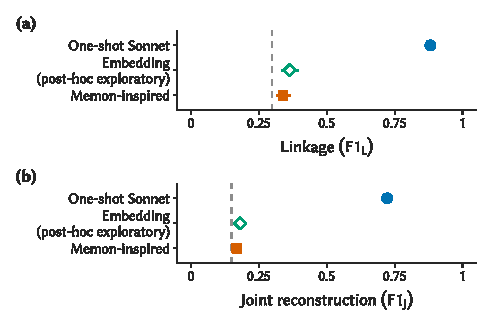
\includegraphics{fig1_headline_attackers.pdf}
  \caption{Headline attacker comparison, 46 pools. Linkage (a) and joint
  reconstruction (b), with the trivial-strategy reference as a dashed line. The
  embedding row is post-hoc exploratory.}
  \label{fig:headline}
\end{figure}
\input{table2_headline_attackers}

\subsection{Across cutting strategies and granularities}
Figure~\ref{fig:grid} and Table~\ref{tab:grid} give the nine-cell grid. The
cutting strategy moves the result more than the granularity label does: at
matched mean fragment length, random and semantic clause cells differ by
$0.087$ in \AJ\ and the two token-window cells by $0.076$. The most disruptive
cut (subject-verb, clause) gives $\FJ = 0.498$ against $0.739$ for
semantic/sentence.

\begin{figure}[t]
  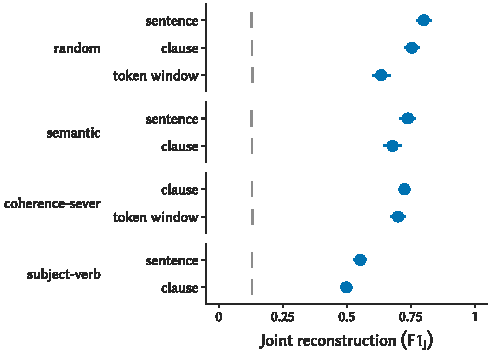
\includegraphics{fig2_grid_reconstruction.pdf}
  \caption{Reconstruction across four cutting strategies and three granularity
  labels.}
  \label{fig:grid}
\end{figure}
\input{table3_grid}

\subsection{Which half fails}
Figure~\ref{fig:decomp} separates the two components. Linkage is the stronger
signal throughout the prose grid; conditional ordering degrades first as the cut
becomes more disruptive.

\begin{figure}[t]
  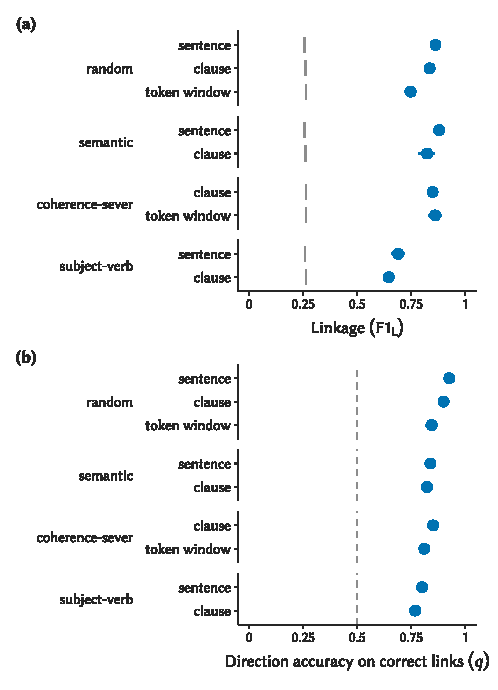
\includegraphics{fig3_linkage_vs_ordering.pdf}
  \caption{The joint score split into linkage and conditional ordering.}
  \label{fig:decomp}
\end{figure}

\subsection{Ordering when membership is given}
With membership supplied (Game~O), the generative attacker orders the headline
documents at $\tau = 0.769$, i.e.\ $88.5\%$ of pairs correctly ordered, while the
tested lexical orderers sit at chance ($\tau = -0.005$ and $0.012$; random is
$0.000$ by construction). Table~\ref{tab:gameO} and Figure~\ref{fig:gameO} report
this. Read with the caution of \S\ref{sec:setup}: the lexical orderers' similarity
is sparse on this corpus.

\begin{figure}[t]
  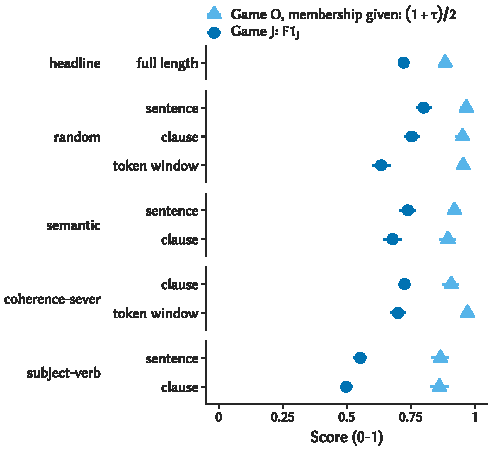
\includegraphics{figA_gameO_vs_gameJ.pdf}
  \caption{Ordering with membership given, against joint recovery.}
  \label{fig:gameO}
\end{figure}
\input{table4_gameO}

\subsection{Structured identifiers behave differently}
\label{sec:identifiers}
On the identifier corpus every content-based attacker falls \emph{below} the
trivial-strategy reference---generative $\AJ = -0.019$, statistical $-0.051$,
embedding $-0.051$, random $-0.049$---while the schema-order baseline, which uses
field structure rather than content, is the only entry above it at $\AJ =
+0.111$. Format leaks here; content does not. This is the clearest evidence in
the study that the effect is a property of the surviving signal rather than of
the attacker.

We state the inference carefully. Prose and identifiers differ in data type,
schema, fragment form and signal structure simultaneously. The contrast is
\emph{consistent with} reconstruction depending on the kind of linkage signal the
fragments preserve; it is not a controlled isolation of ``semantics'' as a causal
variable.

\begin{figure}[t]
  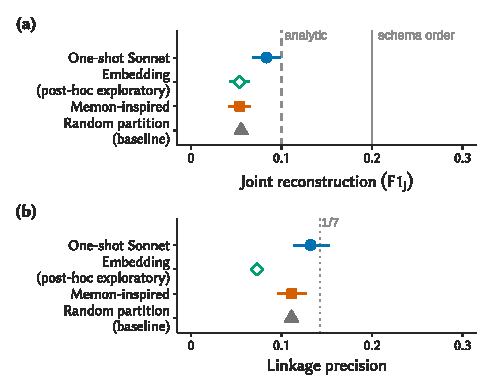
\includegraphics{fig4_identifiers.pdf}
  \caption{The structured-identifier arm.}
  \label{fig:identifiers}
\end{figure}
\input{table5_identifiers}

\subsection{The single-token edge case}
\textbf{Post-hoc exploratory.} On 20 pools and 140 four-sentence excerpts, with
byte-identical text in both arms, cutting at single tokens drives null-adjusted
visible joint reconstruction from $\AVJ = 0.588$ to $0.016$---a paired difference
of $0.572$ $[0.539, 0.607]$, positive in 20 of 20 pools, sign test
$p = 1.9\times10^{-6}$.

\begin{figure}[t]
  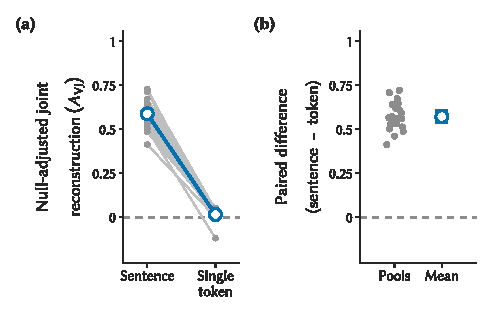
\includegraphics{fig5_single_token.pdf}
  \caption{Post-hoc exploratory single-token edge case.}
  \label{fig:singletoken}
\end{figure}
\input{table6_single_token}

\subsection{A granularity series on identical text}
\label{sec:gradient}
\textbf{Post-hoc exploratory.} Extending that pair to five cuts of the same
excerpts---sentence, four words, three words, two words, one word---gives a
monotone series (Figure~\ref{fig:gradient}, Table~\ref{tab:gradient}):
$\AVJ = 0.588, 0.350, 0.257, 0.127, 0.016$.

Two things must be read with it. First, \textbf{the random-shuffle reference is
not constant across arms}: it falls from $0.423$ at the sentence cut to $0.141$
at one word, so raw \VJ\ is not comparable between arms and the normalised column
is the one to read. Second, the identifier-level score tracks the same shape but
sits below it throughout, and at one word the two fall on \emph{opposite sides}
of their respective references ($+0.016$ visible against the permutation null,
$-0.017$ identifier-level against the one-bucket reference). That divergence is
exactly what the visible scorer exists to handle.

\begin{figure}[t]
  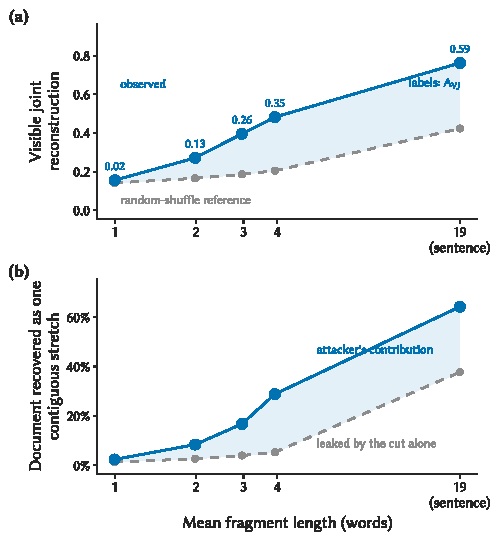
\includegraphics{fig6_granularity_gradient.pdf}
  \caption{Five cuts of identical text. (a) Observed visible joint reconstruction
  against the random-shuffle reference for the same arm, with \AVJ\ printed at
  each point. (b) How much of the 76-word excerpt comes back as one contiguous
  stretch, against the floor leaked by the cut alone.}
  \label{fig:gradient}
\end{figure}
\input{table8_gradient}

\paragraph{The dial has two regimes.}
Panel~(b) separates what the cut gives away from what the attacker earns. At the
sentence cut the attacker ends up holding $64.2\%$ of the document as one
contiguous stretch---but $37.7$ points of that are a single fragment, leaked by
the cut before any reconstruction happens. Join recall, the share of true
adjacent joins recovered, is essentially unchanged between the sentence cut and
the four-word cut ($0.464$ versus $0.476$) while recovered text falls from
$64.2\%$ to $28.8\%$. Across that range, protection comes from reducing what is
free, not from the attacker performing worse. Below four words the attacker's own
joining ability is what fails: join recall falls to $0.315$, $0.153$, $0.022$.

\subsection{What the score means: precedence against adjacency}
\label{sec:adjacency}
\FJ\ counts every within-document precedence pair, not immediate adjacency, and
the gap between those is large. On the headline pools the generative attacker
scores $\FJ = 0.723$ but an immediate-adjacency $F_1$ of $0.287$, with a longest
intact run of $4.53$ fragments. The honest reading is that the attacker recovers
source association and broad relative order well, and contiguous plaintext much
less well. Table~\ref{tab:adjacency} reports this together with a random attacker
that is a \emph{legal} answer to the game.

That random attacker also corrects the reference. A size-blind random partition
into seven groups scores $\FJ = 0.077$, against the one-bucket figure of $0.149$:
the trivial-strategy reference overstates the floor by roughly a factor of two,
and \AJ\ correspondingly understates the advantage over a legal random attacker.
The non-generative attackers collapse on this surface in a way the precedence
score hides---adjacency $F_1$ of $0.010$ and $0.011$ against a random $0.004$,
with about five of seven documents returning no correct adjacency at all.

\input{table9_adjacency}

\subsection{Resources}
Figure~\ref{fig:resources} and Table~\ref{tab:resources} report output scaling,
completion and cost. Output grows with fragment count, but fragment count does
not determine completion: exactly one of 652 prespecified units reached the
output budget.

\begin{figure}[t]
  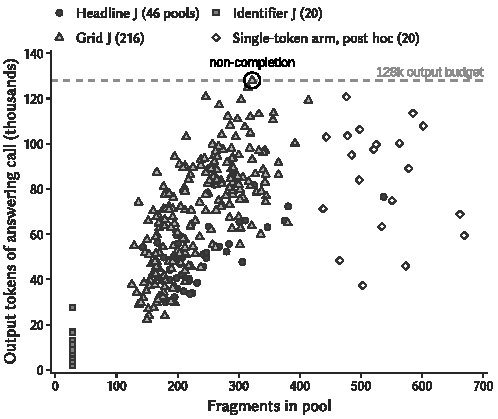
\includegraphics{figB_resource_scaling.pdf}
  \caption{Output scaling and completion.}
  \label{fig:resources}
\end{figure}
\input{table7_resources}

% =====================================================================
\section{Discussion}
\label{sec:discussion}

\paragraph{What the result is.}
Disjointness did not remove the dependency. On clinical prose cut at sentence
granularity, an attacker holding nothing but shuffled plaintext recovers most of
the membership structure and most of the relative order. The channel is the
content itself, which is precisely the dependency that attribute-level
formulations of the problem do not enumerate.

\paragraph{What the result is not.}
It is not a demonstration that fragmentation fails. The same measurement shows
three regimes in which it works. Disruptive cuts reduce the advantage
substantially; structured identifiers defeat every content-based attacker we
tested; and fine granularity drives the score to its reference. Fragmentation's
protection is better understood as conditional on what the fragments retain than
as a property of fragmentation itself---though, as \S\ref{sec:gradient} shows,
the cut strategy and granularity demonstrably matter too, so neither framing
alone is right.

\paragraph{A practical reading.}
For a practitioner the two-regime finding is the useful part. In the coarse
range, finer cutting helps mainly by reducing what is handed over for free; a
sentence-sized fragment \emph{is} a sentence of readable text whatever the
attacker does. Below roughly four words on this corpus, finer cutting begins to
defeat the attacker itself. We deliberately do not convert this into a
recommended fragment size (\S\ref{sec:limitations}).

\paragraph{Interpreting the headline number.}
We would discourage reading $\FJ = 0.723$ as ``$72\%$ of the document was
reconstructed''. It is an $F_1$ over directed within-document pairs. The
corresponding immediate-adjacency score is $0.287$ and the longest intact run is
$4.53$ fragments. Both belong in any summary of this work.

\subsection{Limitations}
\label{sec:limitations}

\textbf{One corpus, one model, one closed world.} All prose results come from a
single corpus of clinical case reports and a single attacker model. External
validity beyond that is not established.

\textbf{$N$ is fixed and unswept.} The number of mixed sources is held at seven
throughout. Prior work in both neighbouring literatures varies the analogous
parameter---pool size and match prior in~\cite{lermen2026}, the number of mixed
documents in~\cite{paixao2020}---and we do not. Whether and how the result moves
with $N$ is open, and we caution that results from a visual channel do not
transfer to a semantic one.

\textbf{The tested baselines are not a competitive frontier.} The statistical and
lexical attackers are implementations we chose; their weakness bounds nothing
about what a stronger classical attacker could do.

\textbf{The granularity series is post hoc.} It was designed after the first
results were seen, is labelled as such throughout, and uses one cut family
(fixed word width) on one corpus. It locates where the advantage falls to its
reference on the tested excerpts. \textbf{It does not establish a safe fragment
size}, and the integer widths tested should not be interpolated.

\textbf{The reference points are imperfect.} The one-bucket reference is a
trivial-strategy benchmark that is not itself a legal answer, and overstates the
floor by roughly a factor of two relative to a legal random partition
(\S\ref{sec:adjacency}). Results normalised against it understate the advantage.

\subsection{Synthetic data}
\label{sec:synthetic}
\textbf{The identifier arm is evaluated entirely on synthetic records} from a
seeded generator; no record corresponds to a person. We argue the extrapolation
narrowly. The arm's role is a contrast, not an estimate: it tests whether a
content-based attacker that succeeds on prose also succeeds when the fragments
carry schema regularities instead of narrative meaning. That comparison depends
on the \emph{structure} of the records---field types, field order, format
regularity---which the generator reproduces faithfully and which is the property
the schema-order baseline exploits. It does not depend on the particular names or
numbers, which is why synthetic values are adequate here.

What the arm does \emph{not} support is any quantitative claim about real
identifier databases: real records carry correlations between fields (a surname
and a country, a date and a record identifier) that a seeded generator does not
reproduce, and those correlations are exactly the kind of dependency this paper
shows can be exploited. We therefore read the identifier result only as evidence
that \emph{this} attacker's advantage on prose does not transfer to
schema-dominated fragments, and not as evidence that identifier fragmentation is
safe. \TODO{authors: confirm this is the argument you want to make, and that it
satisfies the venue's synthetic-data requirement}

% =====================================================================
\section{Conclusion}
Fragmentation removes explicit associations, but disjointness does not remove the
dependencies that let those associations be reconstructed. That insufficiency is
established for declared, attribute-level dependencies; we asked whether the
implicit dependencies carried by natural-language content constitute a comparable
channel, in a setting where the physical, visual and overlap evidence used by
prior reconstruction work is unavailable. On clinical prose, a modern semantic
attacker recovers substantial source association and relative order from
plaintext fragments alone. The effect is conditional: it weakens with disruptive
cuts, disappears on structured identifiers against every content-based attacker
we tested, and falls monotonically to its reference as fragments shrink. We
report the measurement and its decomposition, not a new reconstruction method,
and not a safe fragment size.

% =====================================================================
\begin{acks}
\TODO{author contributions in the agreed form; funding; competing interests}
\end{acks}

\begin{ethics}
This study attacks documents that are already public: the prose corpus is drawn
from open-access literature under commercial-use licences, and the identifier
corpus is synthetic, with no record corresponding to a person. No private data
was accessed, no system was attacked, and no individual is re-identified by any
result reported here. The reconstruction capability we measure is a property of
widely available models rather than a technique we introduce, and we publish it
because designers of fragmentation schemes cannot reason about a channel they
have not been shown. We release the measurement harness and the frozen analysis
rather than a packaged attack tool. \TODO{authors: confirm IRB/exempt status
language and any institutional requirement}
\end{ethics}

\begin{openscience}
The harness, cutters, attackers, scoring code, decision log and the frozen
analysis artifacts behind every figure and table are released at \TODO{repository
URL}. Each figure ships the exact data frame it was plotted from, and the figure
build ends in an independent validation pass that checks every plotted value
against the frozen sources. The prose corpus is reproducible from the published
identifiers and the retrieval scripts; the identifier corpus is reproducible from
its seed. Model outputs are included so the scoring can be re-run without
re-purchasing inference. \TODO{confirm what can be released, and the licence}
\end{openscience}

\begin{ai}
An AI assistant with access to the project's decision log, frozen results and
figure package produced a complete reference draft of this paper, which the
authors used to see one possible shape of the argument before writing their own.
The submitted manuscript is the authors' own prose. \TODO{authors: name any
section that retains drafted text, or state that none does.} AI assistance was
also used during the research itself: for code review and implementation support
in the harness and analysis, for literature retrieval and verification, and for
generating figure and table code. All experimental design decisions, the
pre-registration, the decision log and the interpretation of results are the
authors'. The attacker under study is itself a language model; its use is the
object of the experiment and is described in \S\ref{sec:setup}.
\end{ai}

\bibliographystyle{ACM-Reference-Format}
\bibliography{refs}

\appendix
\section{Additional results}
\input{table1_design}
\begin{figure}[t]
  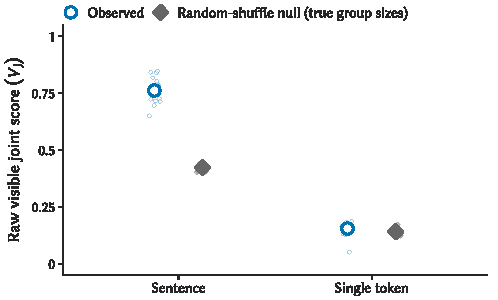
\includegraphics{figC_token_raw_vs_null.pdf}
  \caption{Post-hoc exploratory: observed against null in raw terms.}
  \label{fig:rawnull}
\end{figure}

\end{document}
